\documentclass[]{article}
\usepackage{geometry}
\geometry{a4paper, margin=1in}
\usepackage{amssymb}
\usepackage{multirow}                                                      % you want to use the \thanks command
%\usepackage{multicolumn}
\usepackage{amsmath}
\usepackage{amsfonts}
%\usepackage{math}
\usepackage{adjustbox}
%\usepackage{graphics}
\usepackage{subfigure}
\setcounter{tocdepth}{3}
\usepackage{graphicx}
\usepackage{xcolor}
%\usepackage{url,hyperref,lineno,microtype}
%\usepackage[onehalfspacing]{setspace}
%\usepackage{amssymb}
%\usepackage{subfigure}
%\usepackage{bm}
%\usepackage{multirow}
\usepackage{amsbsy}
%\usepackage{color}
%\usepackage{cite}
%\setcounter{tocdepth}{3}
%\usepackage{graphicx}

\newcommand{\tr}{\operatorname{tr}}
\newcommand{\gD}[2]{\mathcal{N}\left(#1,#2\right)}
\newcommand{\dWj}{\partial\projMat}
\newcommand{\kernel}[2]{k\left(#1,#2\right)}
\newcommand{\kernelww}[2]{k\left(\mathbf{w}_{#1}^d,\mathbf{w}_{#2}^d\right)}
\newcommand{\kernelwx}[1]{k\left(\mathbf{w}_{#1}^d,\indobj\right)}
\newcommand{\catD}[2]{\mathcal{G}\left(#1,#2\right)}
\newcommand{\Z}{\boldsymbol{\mathrm{Z}}}
\newcommand{\C}{\boldsymbol{\Lambda}_j}
\newcommand{\Cin}{\mathbf{C}_j}
\newcommand{\muJ}{\boldsymbol{\mu}_j}
\newcommand{\gammaA}{\Gamma\left(a\right)}
\newcommand{\eye}{\mathbf{I}}
\newcommand{\Scluster}{\mathbf{S}}
\newcommand{\W}{\boldsymbol{\mathcal{W}}}

\newcommand{\WIn}{\mathbf{W}}

\newcommand{\setX}{\mathbf{X}}
\newcommand{\setObj}{\mathbf{X}_d}
\newcommand{\indobj}{\mathbf{x}_{dn}}
\newcommand{\projMat}{\boldsymbol{\mathcal{W}}_d}

\newcommand{\projMatI}{\mathbf{W}_d}
\newcommand{\dWjIn}{\partial\projMatI}
\newcommand{\lvecI}{\mathbf{z}_j}
\newcommand{\lvecsI}{\mathbf{z}_{s_{dn}}}
\newcommand{\lvec}{\boldsymbol{\zeta}_j}
\newcommand{\lvecs}{\boldsymbol{\zeta}_{s_{dn}}}
\newcommand{\mixwe}{{\theta}_j}
\newcommand{\mapphi}{\phi\left(x\right)}
\newcommand{\mapphit}{\phi\left(x'\right)}
\newcommand{\comment}[2]{{\color{blue}#1} {\color{red}#2}}
\newcommand{\phixnd}{\boldsymbol{\phi}\left(\indobj\right)}
\newcommand{\phiwld}[1]{\boldsymbol{\varphi}\left(\mathbf{w}_{#1}^d\right)}
\newcommand{\phiwldI}[2]{\varphi_{#2}\left(\mathbf{w}_{#1}^d\right)}
\newcommand{\wH}{\boldsymbol{\omega}_{j}^d}
\newcommand{\wHj}[1]{\boldsymbol{\omega}_{#1}^d}
\newcommand{\wIj}[1]{\mathbf{w}_{#1}^d}
\newcommand{\muJFa}{\sum_{d=1}^{D}\mathbf{\hat{k}}_d }
\newcommand{\kawx}{\mathbf{\hat{k}}_d }
\newcommand{\Kaww}{\mathbf{\hat{K}}_d }
\newcommand{\dWd}{\partial \boldsymbol{\Theta}}
\newcommand{\likel}{\log p\left(\boldsymbol{\Phi},\mathbf{S}|\W,a,b,r,\gamma\right)}
\newcommand{\GP}[2]{\mathcal{GP}\left(#1,#2\right)}

%\everymath{\displaystyle}
%\everymath{\scriptstyle}
%opening
\title{Probabilistic latent variable models for shape correspondence analysis: Model Approaches}
\author{Hern\'an F. Garc\'ia and Mauricio A. \'Alvarez}

\begin{document}

\maketitle

\begin{abstract}
Probabilistic approaches for the correspondence problem.
\end{abstract}

\section{The model}

Based on the Iwatta's paper (see \cite{Iwata13,Iwata16}), we set nonlinear approaches for the shape correspondence analysis using probabilistic latent variable models.

Suppose that we are given objects in $D$ domains $\mathcal{X}=\left\{\setObj\right\}_{d=1}^D$ mapped to a Hilbert space $\mathcal{H}$, where $\setObj = \left\{\indobj\right\}_{n=1}^{N_d}$ is a set of objects in the $d$th domain, and $\indobj \in \mathbb{R}^{M_d}$ is  the observed vector of the $n$th object in the $d$th domain. We can cluster groups of correspondences by using a non-linear function that represents the shape descriptors in the Hilbert space.

%Our notation is summarized in Table \ref{tab:not}. Note that we are unaware of any correspondence between objects in different domains. The number of objects $N_d$ and the dimensionality $L_d$ for each domain in $\mathcal{H}$ can be different from those of other domains.  Therefore, our task is to match clusters of descriptors (groupwise correspondences) across multiple brain structures in an
%unsupervised manner \cite{Iwata16}.
%
%\begin{table}
%\centering
%\caption{Notation.}
%\label{tab:not}
%\resizebox{\textwidth}{!}{
%\begin{tabular}{l l l}
%\hline
%Symbol in $\mathcal{I}$& Symbol in $\mathcal{H}$  & Description \\
%\hline
%$D$ & &Number of shapes \\
%$N_d$ && Number of objects ($3D$-landmarks) in the $d$th shape\\
%$M_d$ &$L_d$& Dimensionality of the observed features in the $d$th shape\\
%$K$ & $P$ & Dimensionality of a latent vector\\
%$J$ & $Q$ & Number of correspondences (latent vectors) to which objects are assigned\\
%$\indobj$ & $\phixnd$ & Observation of the $n$th object in the $d$th shape, $\indobj \in \mathbb{R}^{M_d}$\\
%$\mathbf{z}_j$  &$\lvec$& Latent vector for the $j$th correspondence, $\lvec \in \mathbb{R}^{K}$ \\
%$\mathbf{W}_d $ &$\projMat$& Projection matrix for the $d$th domain, $\mathbf{W}_d \in \mathbb{R}^{M_d \times K}$ \\
%$\mixwe$ && Mixture weight for the  $j$th cluster, $\mixwe \ge 0$, $\sum_{j=1}^{\infty}{\mixwe} = 1$\\
%\hline
%\hline 
%\end{tabular}}
%\end{table}
%%

As in infinite Gaussian mixture models, our approach assumes that there are an infinite number of clusters related to each
correspondence, and each cluster $j$ has a latent vector $\lvecI\in \mathbb{R}^K$ in a latent space of dimension $K$. Descriptors that have the same cluster assignments $s_{dn}$ are related by the same latent vector and considered to match (establish a groupwise correspondence).

Each object in $\indobj \in \mathcal{R}^{M_d}$ in the $d$th domain is generated depending on the domain-specific projection matrix $\projMatI \in \mathbb{R}^{M_d \times K}$ and latent vector $\lvecsI$ that is selected from a set of latent vectors $\Z = \left\{\lvecI\right\}_{j=1}^\infty$. Here, $s_{dn}=\left\{1,\dots,\infty\right\}$ is the latent cluster assignment of object $\indobj$.


The proposed model is based on an infinite mixture model, where the
probability of descriptor mapped in a Hilbert space $\indobj$ is given by

\begin{equation}
p\left( {{\indobj}|{\Z},{\boldsymbol{{W}}},{\boldsymbol{\theta }}} \right) = \sum\limits_{j = 1}^\infty  {{\theta _j}\mathcal{N}\left(\indobj|\projMatI\lvecI,\alpha^{-1}\mathbf{I}\right)}, 
\label{eq:llNLmodel}
\end{equation}

where $\boldsymbol{{W}} = \left\{\projMatI \right\}_{d=1}^{D}$ is a set of projections
matrices, $\boldsymbol{\theta}=\left(\theta_j\right)_{j=1}^{\infty}$
are the mixture weights, $\theta_j$ represents the probability that
the $j$th cluster is chosen, and
$\mathcal{N}\left(\boldsymbol{\mu},\boldsymbol{\Sigma}\right)$ denotes
a normal distribution with mean $\boldsymbol{\mu}$ and covariance
matrix $\boldsymbol{\Sigma}$. One important contribution derived in \cite{Iwata13}, is that we can analyze multiples structures with different properties and dimensionalities, by employing projection matrices for each brain structure (domain-specific). Figure
\ref{fig:pipeline} shows the scheme of the proposed model, in which
the relationship between shape descriptors, and
latent vectors is described.

\begin{figure}[h!]
\centering
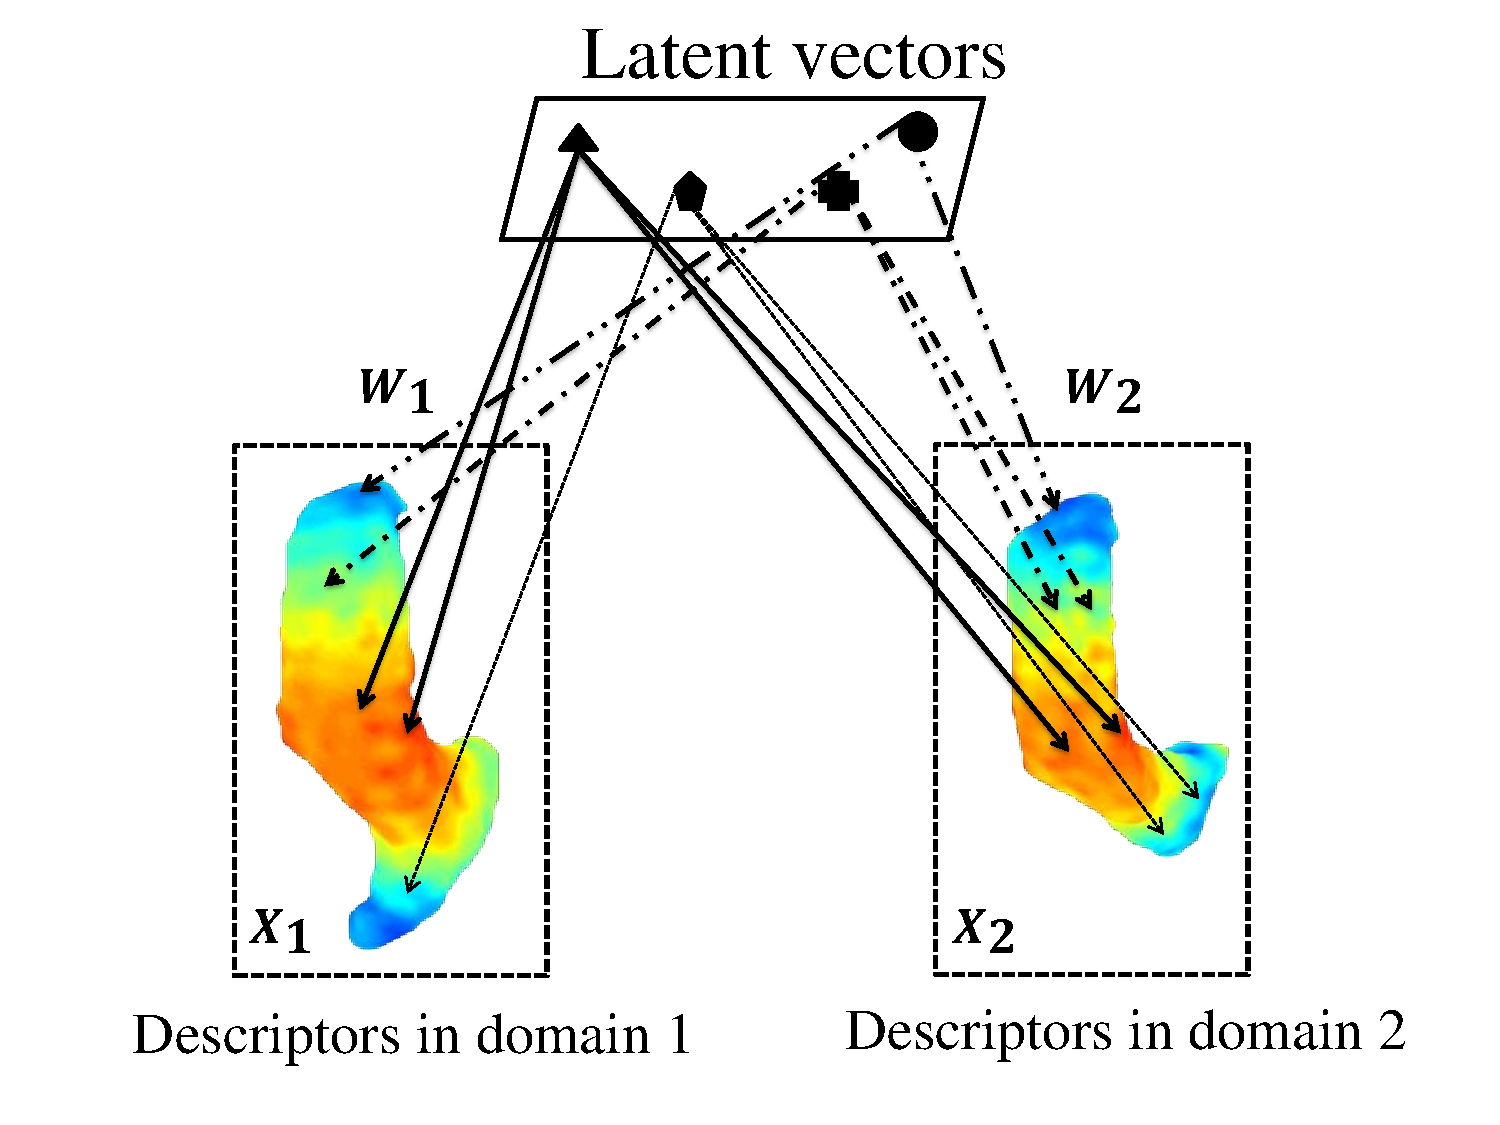
\includegraphics[width=0.6\textwidth]{img/pipelineGroupCorr}
\caption{Scheme for the groupwise correspondence method. The
  figure shows an example of establishing clusters of correspondences
  in two domains (left ventrals).}
\label{fig:pipeline}
\end{figure} 

\section{Model Approaches}

The main ideas for the probabilistic correspondence problem are summarized

\begin{enumerate}
	\item We can relax the assumption that the observations are linear with respect to their latent vectors by using nonlinear matrix factorization techniques (\cite{Lawrence09NMF}). From these work we point out that by marginalizing out the mapping matrix $\mathbf{W}$(which goes
	from the latent space to the observed data space), derived in a Bayesian multi-output regression model. 
	
	Our model can be formalized as
	
	\begin{align}
	p\left( {{\indobj}|{\Z},{\mathbf{{W}}},{\boldsymbol{\theta }}} \right) = \sum_{j=1}^{\infty} \theta_{j}{\prod_{m=1}^{M_d}\gD{\mathbf{x}_{dnm}|f_{dm}\left(\lvecI\right)}{\alpha^{-1}}}
	\end{align}
	
	where $f_{dm}$ can handled from two perspectives
	\begin{enumerate}
		\item Set the same covariance matrix for all domains
		\begin{align}
		f_{dm} \sim \GP{\mu_{dm}\left(\lvecI\right)}{\kernel{\lvecI}{\lvecI'}}
		\end{align}
		
		\item One covariance matrix for each domain
		\begin{align}
		f_{dm} \sim \GP{\mu_{dm}\left(\lvecI\right)}{k_d\left({\lvecI},{\lvecI'}\right)}
		\end{align}
	\end{enumerate}
	
	\item As in the in the linear model of coregionalization (LMC), the outputs are expressed as linear combinations
	of independent random functions \cite{Alvarez12KVF}. Consider a set of $D$ outputs $\left\{\mathbf{f}_d(\mathbf{\lvecI})\right\}_{d=1}^D$
    with $\mathbf{f}_d(\mathbf{\lvecI}) \in \mathbb{R}^{M_d}$. By adopting this framework, our model can be formulated as
    
    \begin{align}
    p\left( {{\indobj}|{\Z},{\mathbf{{W}}},{\boldsymbol{\theta }}} \right) = \sum_{j=1}^{\infty} \theta_j \gD{\indobj|\mathbf{f}_{d}(\mathbf{\lvecI})}{\alpha^{-1}\eye},
    \end{align}
    
    where each component can be expressed as:
    
    \begin{enumerate}
    	\item By using the linear model of coregionalization  
    	\begin{align}
    	\mathbf{f}_d(\mathbf{\lvecI}) \sim \GP{\boldsymbol{0}}{\sum_{q=1}^{Q}\mathbf{B}_q k_d\left(\lvecI,\lvecI'\right)},
    	\end{align}
    	
    	where $\mathbf{B}_q = \mathbf{L}_q^\top\mathbf{L}_q \in \mathbb{R}^{M_d \times M_d}$ is the coregionalization matrix (computed from the Cholesky decomposition)
    	
    	\item By using simplified version of the LMC, known as the intrinsic coregionalization model (ICM) (see \cite{Alvarez12KVF}), assumes that the elements of the coregionalization matrix $\mathbf{B}_q$ can be written as a scaled version of the elements $b_q$, which do not depend on the particular output functions $f_d(\lvecI)$.
    	
    	\begin{align}
    	\mathbf{f}_d(\mathbf{\lvecI}) \sim \GP{\boldsymbol{0}}{\mathbf{B} k\left(\lvecI,\lvecI'\right)},
    	\end{align}
    	
    \end{enumerate}

\end{enumerate}



\section{Multiview Warped Mixture Models}

We can use the single view problem of the warped mixture model from \cite{IwaDuvGha2012warped} in which they warp a latent mixture of Gaussians into nonparametric cluster shapes. The low-dimensional latent mixture model summarizes the properties of the high-dimensional density manifolds describing the data.

Our idea is to introduce a model which warps a multiview latent mixture of Gaussians (possibly MRD) to produce nonparametric cluster shapes. \footnote{The possibly low-dimensional latent mixture model allows us to summarize the properties of the high-dimensional clusters
(or density manifolds) describing the data. The number of manifolds, as well as the shape and dimension of each manifold is automatically inferred.}


\begin{figure}[h!]
	\centering
	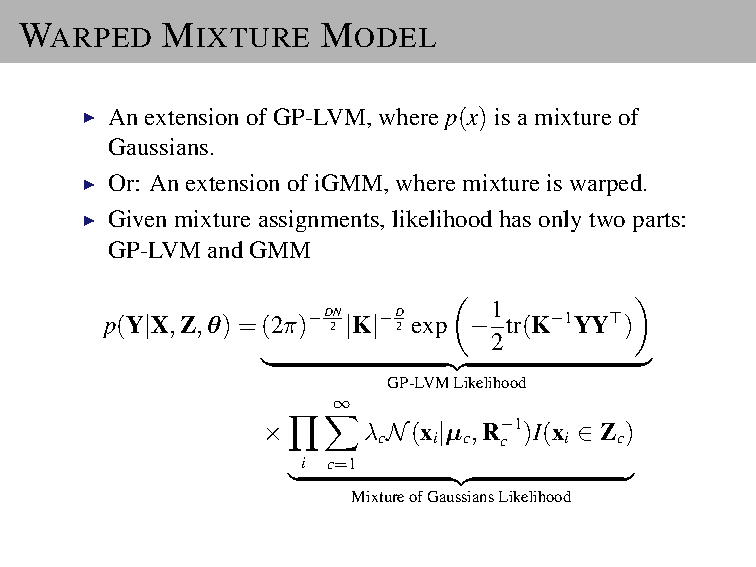
\includegraphics[width=.9\linewidth]{img/iwmm_talk_Model}
	\caption{WMM from \cite{IwaDuvGha2012warped}}
\end{figure}

\subsection{The model}

Let as define a multi-view data set as $\mathcal{Y}=\left\{\mathbf{Y}^{v}\right\}_{v=1}^{V}$, where each view is defined as $\mathbf{Y}^{v}\in \mathbb{R}^{N_v\times D_v}$. This leads to the likelihood

\begin{align}
p\left(\mathbf{Y}^{\mathcal{V}}|\mathbf{X},\mathbf{Z},\boldsymbol{\theta}\right) = \sum_{v=1}^{V}p(\mathbf{Y}^v|\mathbf{X},\boldsymbol{\theta})\times \prod_{i}\sum_{c=1}^{\infty} \lambda_c\gD{\mathbf{x}_i|\boldsymbol{\mu}_c}{\mathbf{R}_c^{-1}} ,\quad \mathbf{x}_i \in \mathbf{Z}_c
\end{align}


Based on the iWMM (see \cite{IwaDuvGha2012warped}) our generative model generates multiple observations $\mathbf{Y}^{\mathcal{V}}$ according to the following generative process:

\begin{enumerate}
	\item Draw mixture weights $\boldsymbol{\lambda}\sim \operatorname{GEM}(\eta)$
	\item For each cluster $c = 1, \cdots,\infty $
	\begin{enumerate}
		\item Draw precision $\mathbf{R}_c \sim \mathcal{W}(\mathbf{S}^{-1},v)$
		\item Draw mean $\boldsymbol{\mu}_c \sim \mathcal{N}(\mathbf{u},(r\mathbf{R}_c)^{-1})$
	\end{enumerate}
	
	\item For each view $v = 1, \cdots,\mathcal{V} $
	\begin{enumerate}
		\item For each observation $n = 1,\cdots,N_v$
	\begin{enumerate}
		\item Draw latent assignment $z_{nv} \sim \operatorname{Mult}(\boldsymbol{\lambda})$
		\item Draw latent coordinates $\mathbf{x}_{nv} \sim \mathcal{N}(\boldsymbol{\mu}_{z_{nv}},\mathbf{R}_{z_{nv}}^{-1})$
	\end{enumerate}
	\end{enumerate}

	\item For each view $v = 1, \cdots,\mathcal{V} $
	\begin{enumerate}
		\item For each observed dimension $d = 1,\cdots,D_v$
		\begin{enumerate}
			\item Draw function $\mathbf{f}_{d}^{v} \sim \mathcal{GP}(\mathbf{0},\mathbf{K}^{v})$
		\end{enumerate}
	\end{enumerate}

	\item For each view $v = 1, \cdots,\mathcal{V} $
	\begin{enumerate}
		\item For each observed dimension $d = 1,\cdots,D_v$
		\begin{enumerate}
			\item For each observed dimension $d = 1,\cdots,D_v$
			\begin{enumerate}
				\item Draw feature $y_{nd}^{v}\sim \gD{\textcolor{red}{\mathbf{W}^v}f_d^{v}(\mathbf{x}_{nv})}{\beta^{-1}}$
			\end{enumerate}
		\end{enumerate}
	\end{enumerate}
\end{enumerate}

We define the dimensionalities of our variables as:

\begin{itemize}
	\item 	$K$: real number of clusters
	\item $Q$:  dimensionality of the Latent Space
	\item $D_v$: dimensionality of the input data in the $v$-th view 
	\item $\boldsymbol{\lambda} \in \mathbb{R}^{K\times 1}$ 
	\item $\mathbf{R}_c \in \mathbb{R}^{Q\times Q}$
	\item $\boldsymbol{\mu}_c \in \mathbb{R}^{Q\times 1}$
\end{itemize}

\bibliographystyle{plain}
\bibliography{bibRevTesisDoc}

\end{document}
